\documentclass[aspectratio=169,12pt,spanish]{beamer}
\usepackage[T1]{fontenc}
\usepackage[spanish]{babel}

\usepackage{wrapfig}

%\usepackage{multicol}
%\usepackage{mathtools}

\usepackage[normalem]{ulem}

\usepackage{pgf,tikz}
\usetikzlibrary{matrix}
\usetikzlibrary{arrows}

%\usepackage{wrapfig}
\mode<presentation>
\usefonttheme{professionalfonts}
\usetheme{Darmstadt}
\usecolortheme{orchid}
\useoutertheme{default}
\setbeamertemplate{headline}{}

\newcounter{savedenum}
\newcommand*{\saveenum}{\setcounter{savedenum}{\theenumi}}
\newcommand*{\resume}{\setcounter{enumi}{\thesavedenum}}

\renewcommand{\baselinestretch}{1.1}

%gets rid of bottom navigation bars
\setbeamertemplate{footline}[page number]

%gets rid of navigation symbols
\setbeamertemplate{navigation symbols}{}

%\frameframe{none} % No default frame

%\setlength{\framewidth}{8.7in} \setlength{\frameheight}{7.2in}

\parindent 0pt
\setlength{\parskip} {1ex plus 0.5ex minus 0.2ex}


\usepackage[bbgreekl]{mathbbol}
\usepackage{amssymb, amsthm, amsmath}
\usepackage{bm}

\newtheorem{ejercicio}{Ejercicio}
\newtheorem{proposition}[theorem]{Proposición}

\DeclareSymbolFontAlphabet{\mathbb}{AMSb}
\DeclareSymbolFontAlphabet{\mathbbl}{bbold}

\usepackage{multicol}
\usepackage{colortbl}
\usepackage{lmodern}
\usepackage{tabularx}
\usepackage{multirow}
\usepackage{stmaryrd}
\usepackage{color}
\usepackage{graphicx}
\usepackage{hyperref}

\graphicspath{ {../../images} }
\usepackage{listings}
\lstset{
  basicstyle=\ttfamily,
  columns=fullflexible,
}

\usepackage{url}
\usepackage{multicol}
\usepackage{dsfont}

% Bold symbols for vectors and matrices
\newcommand{\xstar}{\bm{x}^{\star}}
\newcommand{\alphab}{\bm{\alpha}}
\newcommand{\ab}{\bm{a}}
\newcommand{\bb}{\bm{b}}
\newcommand{\cb}{\bm{c}}
\newcommand{\db}{\bm{d}}
\newcommand{\eb}{\bm{e}}
\newcommand{\gb}{\bm{g}}
\newcommand{\mb}{\bm{m}}
\newcommand{\pb}{\bm{p}}
\newcommand{\qb}{\bm{q}}
\newcommand{\rb}{\bm{r}}
\newcommand{\ssb}{\bm{s}}
\newcommand{\ub}{\bm{u}}
\newcommand{\vb}{\bm{v}}
\newcommand{\wb}{\bm{w}}
\newcommand{\xb}{\bm{x}}
\newcommand{\yb}{\bm{y}}
\newcommand{\zb}{\bm{z}}

\newcommand{\Ab}{\bm{A}}
\newcommand{\Bb}{\bm{B}}
\newcommand{\Cb}{\bm{C}}
\newcommand{\Db}{\bm{D}}
\newcommand{\Eb}{\bm{E}}
\newcommand{\Fb}{\bm{F}}
\newcommand{\Gb}{\bm{G}}
\newcommand{\Hb}{\bm{H}}
\newcommand{\Ib}{\bm{I}}
\newcommand{\Id}{\bm{I}}
\newcommand{\Kb}{\bm{K}}
\newcommand{\Lb}{\bm{L}}
\newcommand{\Mb}{\bm{M}}
\newcommand{\Pb}{\bm{P}}
\newcommand{\Qb}{\bm{Q}}
\newcommand{\Rb}{\bm{R}}
\newcommand{\Sb}{\bm{S}}
\newcommand{\Tb}{\bm{T}}
\newcommand{\Ub}{\bm{U}}
\newcommand{\Vb}{\bm{V}}
\newcommand{\Wb}{\bm{W}}
\newcommand{\Xb}{\bm{X}}
\newcommand{\Yb}{\bm{Y}}
\newcommand{\Zb}{\bm{Z}}
\newcommand{\Lambdab}{\bm{\Lambda}}
\newcommand{\cero}{\bm{0}}

% Rings and fields
\newcommand{\A}{\mathbb{A}}
\newcommand{\Z}{\mathbb{Z}}
\newcommand{\Q}{\mathbb{Q}}
\newcommand{\C}{\mathbb{C}}
\newcommand{\R}{\mathbb{R}}
\newcommand{\K}{\mathbb{K}}
\newcommand{\N}{\mathbb{N}}

\newcommand{\borel}{{\mathcal B}}
\newcommand{\pmom}{{\rho_{\text{mom}}}}
\newcommand{\MX}{{\mathcal{M}(X)}}


% Inner product
\newcommand{\innerl}[2]{\langle #1, #2 \rangle}
\newcommand{\inner}[2]{#1 \boldsymbol{\cdot} #2}
\newcommand{\innerTrace}[2]{#1 \bullet #2}

% Symmetric and positive definite matrices
\newcommand{\Splusplusn}{{\mathcal S_{++}^n}}
\newcommand{\Splusn}{{\mathcal S_+^n}}
\newcommand{\Splus}{{\mathcal S_+}}
\newcommand{\Sym}{{\mathcal S}}
\newcommand{\Symn}{{\mathcal S^n}}

% Cones
\newcommand\CC{\mathcal{C}}
\DeclareMathOperator{\cone}{cono}
\DeclareMathOperator{\conv}{conv}
\DeclareMathOperator{\supp}{supp}


% Spectrahedron
\newcommand{\eLL}{{\mathcal L}}

% Matrices and vectors over R or C
\newcommand{\Rnn}{\R^{n\times n}}
\newcommand{\Cnn}{\C^{n\times n}}
\newcommand{\Rn}{\R^{n}}
\newcommand{\Rm}{\R^{m}}


% Math operators
\DeclareMathOperator{\Tr}{Tr}
\DeclareMathOperator{\tr}{Tr}
\DeclareMathOperator{\interior}{int}
\DeclareMathOperator{\rank}{rank}
\DeclareMathOperator{\diag}{diag}

\newcommand\one{\mathds{1}} 

\pagestyle{empty}

\begin{document}

%------------------------------------------------------------------

\begin{frame}

 \begin{center}

\Large\textbf{Optimización Semidefinida} \\
\large\textbf{Clase 11 - Distancia euclídea y rango mínimo}
%\vspace{0.5cm}

% \textit{Santiago Laplagne} \\
%slaplagn@dm.uba.ar \\


%\vspace{0.5cm}
%{\small Trabajo en progreso en conjunto con \emph{Jose Capco} (Universit\"at Innsbruck) y \emph{Claus Scheiderer} %(Universit\"at Konstanz).} \\

\vspace{1cm}
 Segundo Cuatrimestre 2021
 \\
 {\small Facultad de Ciencias Exactas y Naturales, UBA}
 \end{center}

\end{frame}



%------------------------------------------------------------------

\begin{frame}
\frametitle{Distancias euclídeas}

Consideramos un grafo $G = (N, E)$ con nodos $N = \{1, \dots, n\}$, aristas $E \subset N \times N$, y pesos no negativos $D = \{d_{ij}\} \in \R_+^E$, que representan distancias entre los nodos.

Decimos que $(G, D)$ es $k$-realizable si podemos ubicar los nodos de $G$ en puntos $\vb_1, \dots, \vb_n \in \R^k$ de forma tal que las distancias euclídeas entre los nodos respeten las longitudes dadas:
$$
\exists \vb_1, \dots, \vb_n \in \R^k:  \| \vb_i - \vb_j \| = d_{ij} \quad \forall \{i, j\} \in E.
$$

Decimos que $(G, D)$ es realizable (a secas) si existe $k$ tal que $(G, D)$ es $k$-realizable.

\end{frame}

%------------------------------------------------------------------

\begin{frame}
\frametitle{Grafo completo}

Para el caso de un grafo completo tenemos la siguiente caracterización.

\begin{theorem}
Sea $G = K_n$ un grafo completo, con pesos $D$, y sea $\Ab \in \Sym^{n}$ la matriz
{\small
$$
\Ab = \begin{pmatrix}
0 & d_{21}^2 & d_{31}^2 & \dots & d_{n1}^2 \\
d_{21}^2 & 0 & d_{32}^2 & \dots & d_{n2}^2 \\
\vdots & \vdots & \vdots & \ddots & \vdots \\
d_{n1}^2 & d_{n2}^2 & d_{n3}^2 & \dots & d_{nn}^2
\end{pmatrix}
$$}
\vspace{-0.5cm}

El grafo $G$ es realizable si y solo si $\Ab$ es semidefinida negativa en el espacio ortogonal al vector $\eb = (1, 1, \dots, 1)$. Es decir, si
$$
\yb^T \Ab \yb \le 0 \quad \text{ para todo } \yb \in \R^n \text{ tal que } \sum_{i=1}^n y_i = 0.
$$
\end{theorem}

\end{frame}

%------------------------------------------------------------------

\begin{frame}
\frametitle{Demostración}

Demostramos solo $\Rightarrow$.

Suponemos que existen vectores $\vb_i \in \R^k$ para algún $k \ge 1$ tales que $d_{ij} = \|\vb_i - \vb_j\|$. Consideramos ahora la matriz $\Xb$ de productos internos
$$
\Xb = \begin{pmatrix}
\innerl{\vb_1}{\vb_1} & \innerl{\vb_1}{\vb_2} & \dots & \innerl{\vb_1}{\vb_n} \\
\innerl{\vb_2}{\vb_1} & \innerl{\vb_2}{\vb_2} & \dots & \innerl{\vb_2}{\vb_n} \\
\vdots & \vdots & \ddots & \vdots \\
\innerl{\vb_n}{\vb_1} & \innerl{\vb_n}{\vb_2} & \dots & \innerl{\vb_n}{\vb_n}
\end{pmatrix} = (\vb_1 \dots \vb_n)^T (\vb_1 \dots \vb_n),
$$
que es semidefinida positiva. Como $a_{ij} = \| \vb_i - \vb_j\|^2 = \innerl{\vb_i}{\vb_i} + \innerl{\vb_j}{\vb_j} - 2 \innerl{\vb_i}{\vb_j}$, tenemos
$$
\Ab = \inner{\diag(\Xb)}{\eb^T} + \inner{\eb}{\diag(\Xb)} - 2 \Xb.
$$

Por lo tanto, para $\yb \perp \eb$, $\yb^T \Ab \yb = -2 \yb^T \Xb \yb \le 0$.


\end{frame}


%------------------------------------------------------------------

\begin{frame}
\frametitle{Grafos no completos}

En general, para grafos no completos determinar si el grafo es realizable equivale a buscar una solución factible de un problema SDP.

\begin{theorem}
Un grafo con pesos $(G, D)$ es realizable si y solo si el siguiente problema SDP tiene solución
\begin{alignat*}{2}
  & \text{existe: } & & \Xb \in \Sym^n \\
   & \text{sujeto a: } & \quad & x_{ii} + x_{jj} - 2 x_{ij} = d_{ij}^2 \quad \forall \{i, j\} \in E, \\
   &&& \Xb  \succeq 0
\end{alignat*}

Más aún, $(G, D)$ es $k$-realizable si existe una solución $\Xb$ de rango a lo sumo $k$.
\end{theorem}

\end{frame}

%------------------------------------------------------------------

\begin{frame}
\frametitle{Demostración}

Si $\vb_1, \dots, \vb_n \in \R^k$ es una realización de $(G, D)$, entonces la matriz de Gram
$$
\Xb = (\innerl{\vb_i}{\vb_j}) = (\vb_1 \dots \vb_n)^T (\vb_1 \dots \vb_n)
$$
es una solución del problema, de rango a lo sumo $k$.

Recíprocamente, si $\Xb$ es una solución del problema, podemos encontrar una descomposición
$$
\Xb = \Vb^T \Vb, \quad \Vb \in \R^{k \times n}
$$
y tomamos como $\vb_i$ las columnas de $\Vb$.

\end{frame}

%------------------------------------------------------------------

\begin{frame}
\frametitle{Grafos completos revisitados}

Utilizando el último teorema obtenemos otra caracterización para grafos completos.

\begin{theorem}
Sea $G = K_n$ grafo completo, con pesos $D$, y sea $\Xb \in \Sym^{n-1}$ la matriz definida por
\begin{align*}
x_{ii} &= d_{in}^2, \quad \forall 1 \le i \le n-1 \\
x_{ij} &= \frac{d_{in}^2 + d_{jn}^2 - d_{ij}^2}{2}, \quad \forall 1 \le i \neq j \le n-1.
\end{align*}

Entonces $K_n$ es $k$-realizable si y solo si $\Xb \succeq 0$ y $\rank \Xb \le k$.
\end{theorem}

\textbf{Idea de la demostración.} Si el problema SDP tiene solución factible, mediante una traslación, podemos suponer $\vb_n = \cero$.
\end{frame}

%------------------------------------------------------------------

\begin{frame}
\frametitle{El problema de la partición}

Como vimos, determinar si un grafo $(G, D)$ es realizable, puede resolverse eficientemente por optimización semi-definida.
Sin embargo, determinar si es $k$-realizable para un $k$ dado es un problema mucho más difícil.

Veremos un caso simple en el que el problema es NP-completo.

Consideramos el siguiente problema para el cual se sabe que es NP-completo.

\begin{block}{El problema de la partición.}
Dada una secuencia de números naturales $a_1, \dots, a_n \in \N$, determinar si los números pueden separarse en dos conjuntos con la misma suma. Es decir, si existe $\bm{\epsilon} \in \{\pm 1\}^n$ tal que
$$
\epsilon_1 a_1 + \dots + \epsilon_n a_n = 0.
$$
\end{block}

\end{frame}

%------------------------------------------------------------------

\begin{frame}
\frametitle{Grafo ciclo}

Un grafo $(G, E)$ se llama ciclo o cíclico si las aristas forma un ciclo de longitud $n$. Es decir, podemos suponer que las aristas son $(i, i+1)$ para $1 \le i \le n-1$ y $(n, 1)$.

\begin{theorem}
Dado un grafo ciclo $(G, E)$ con pesos naturales $d \in \N^E$, decidir si $(G,D)$ es $1$-realizable es un problema NP-completo.
\end{theorem}

\textbf{Demostración.}

Para una instancia $a_1, \dots, a_n \in \N$ del problema de la partición, consideramos el grafo ciclo $(G,E)$ con pesos $d_{i(i+1)} = a_i$.

Si $(G,D)$ es $1$-realizable, con $v_i \in \R$, definimos $\epsilon_i = 1$ si $v_{i+1} > v_i$ y $\epsilon_i = -1$ si $v_{i+1} < v_i$ y obtenemos una partición de los $a_i$.




\end{frame}

%------------------------------------------------------------------

\begin{frame}
\frametitle{Rango 1 y rango 2}

Puede demostrarse la siguiente propiedad:

\begin{center}
Un grafo ciclo es realizable si y solo si es $2$-realizable.
\end{center}

\textbf{Ejercicio.} Ver geométricamente que puedo llevar una realización 3D de un grafo ciclo a una realización 2D.

Concluimos que es posible contestar eficientemente si un grafo ciclo es realizable en un plano o una recta, pero determinar en cuál de los dos es un problema NP-completo.

\end{frame}

%------------------------------------------------------------------

\begin{frame}
\frametitle{Minimización de rango}

Como vimos, un problema interesante en optimización es el problema de la minimización de rango, que podemos plantear en la forma
\begin{alignat*}{2}
  & \text{minimizar: } & & \rank \Xb  \\
   & \text{sujeto a: } & \quad & \Xb  \in \mathcal{C},
\end{alignat*}
donde la matriz $\Xb \in \R^{m \times n}$ es la variable de decisión, y $\mathcal{C}$ es un conjunto convexo. Como la función a optimizar tiene valores enteros, este problema en general no es un problema convexo. En el ejemplo anterior vimos que en general es un problema NP-completo.

\end{frame}

%------------------------------------------------------------------

\begin{frame}
\frametitle{Ejemplo - El problema de Netflix}

\begin{minipage}[t]{0.65\textwidth}
\begin{itemize}
\item Algunos usuarios califican algunas de las películas que vieron.
\item Los puntajes son números enteros entre 1 y 5.
\item Queremos predecir los puntajes para cada par usuario / película.
\item Es decir, queremos completar una matriz incompleta como la de la figura.
\end{itemize}
\end{minipage}
\begin{minipage}[t]{0.3\textwidth}
\begin{center}
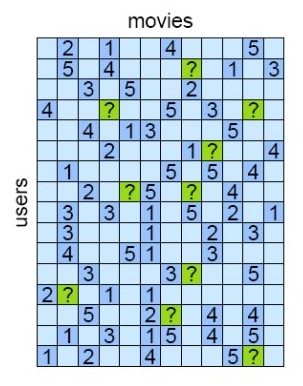
\includegraphics[scale=.6]{rank_netflix.jpg}
\end{center}
\end{minipage}



\end{frame}


%------------------------------------------------------------------

\begin{frame}
\frametitle{Ejemplo - El problema de Netflix}

Si pensamos que hay unos pocos perfiles de usuarios arquetípicos (amante de las películas de terror, románticas, comedias, etc.) y cada usuario es una combinación lineal de esos perfiles, podemos factorizar la matriz:

\begin{center}
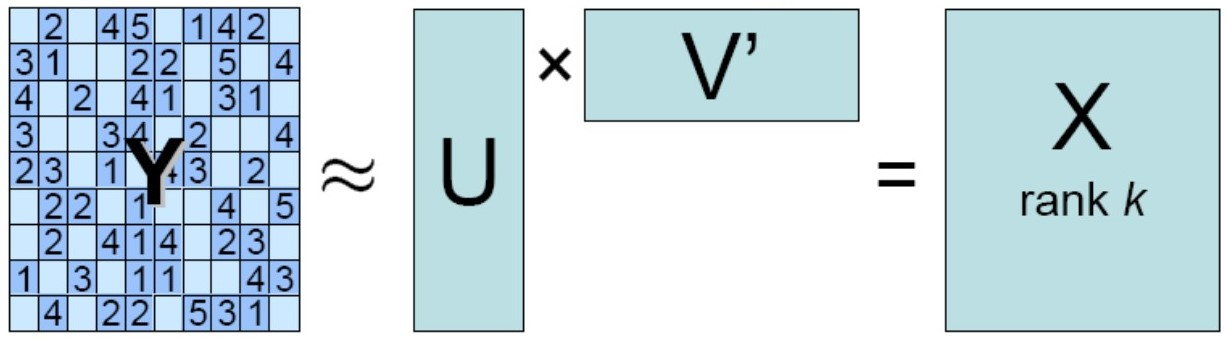
\includegraphics[scale=.4]{rank_factorization.jpg}
\end{center}

\end{frame}

%------------------------------------------------------------------

\begin{frame}
\frametitle{Rango y valores singulares}

\begin{itemize}
\item Para una matriz $\Ab \in \Rnn$ cuadrada, el rango de $\Ab$ es igual a la cantidad de autovalores no-nulos.
\item Para una matriz $\Ab \in \R^{m \times n}$, el rango de $\Ab$ es igual a la cantidad de valores singulares no-nulos.
\end{itemize}

\textbf{Heurística}
\begin{itemize}
\item Como no podemos minimizar el rango eficientemente, minimizamos la suma de los valores singulares.
\item Para $\Ab \succeq 0$, la suma de los valores singulares es igual a $\Tr(\Ab)$, que es una función lineal en los coeficientes de $\Ab$.
\end{itemize}

\end{frame}

%------------------------------------------------------------------

\begin{frame}
\frametitle{Norma nuclear - Heurística}

\begin{minipage}[c]{0.7\textwidth}
En $\R^{m \times n}$ definimos la norma nuclear
$$
\| \Xb \|_* = \sum_{i=1}^{\min\{m, n\}} \sigma_i.
$$

Como los valores singulares son todos no-negativos,
$$
\| \Xb \|_* = \| \bm{\sigma} \|_1.
$$

Comparando las curvas de nivel distintas normas, vemos que minimizando la norma-1 obtenemos en general vectores esparsos con gran cantidad de 0's. Por este motivo es una buena elección para obtener matrices de rango bajo.
\end{minipage}
\begin{minipage}[c]{0.25\textwidth}
\begin{center}
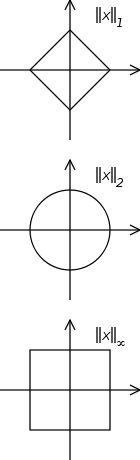
\includegraphics[scale=.4]{140px-Vector_norms.png}
\end{center}
\end{minipage}

\end{frame}

%------------------------------------------------------------------

\begin{frame}
\frametitle{Norma nuclear}


Para analizar las propiedades de la norma nuclear, recordemos las siguientes propiedades:
\begin{itemize}
\item Para $\Ab, \Bb \in \R^{m \times n}$, 
$$\innerTrace{\Ab}{\Bb} = \tr(\Ab^T \Bb)= \tr(\Ab \Bb^T)$$ 
es un producto interno en $\R^{n \times n}$, que define la norma 
$$\|\Ab\|_F = \sqrt{\innerTrace{\Ab}{\Ab}} = \sqrt{\Tr(\Ab \Ab^T)}.$$

Si $\Xb = \Ab \Ab^T$, $\Tr(\Xb) = \|\Ab\|_F^2$.
\item Desigualdad de Cauchy-Schwarz: $|\langle \ub, \vb \rangle| \le \|\ub\| \|\vb\|$
\item Desigualdad MA-MG: $\|\ub\| \|\vb\| \le \frac{1}{2}(\|\ub\|^2 + \|\vb\|^2)$
\end{itemize}

\end{frame}

%------------------------------------------------------------------

\begin{frame}
\frametitle{Norma nuclear}

\begin{lemma}
Para $\Xb \in \R^{n \times n}$, 
$$
\|\Xb\|_* = \min_{\Xb = \Ub \Vb^T} \|\Ub\|_{F} \|\Vb\|_{F} = \min_{\Xb = \Ub \Vb^T} \frac{1}{2}(\|\Ub\|^2 + \|\Vb\|^2).
 $$
\end{lemma}

{\small Este y los siguientes resultados valen también para $\Xb$ rectangular.}

\textbf{Demostración.} Tomamos una descomposición SVD de $\Xb$, 
$$\Xb = \Pb \Sb \Qb^T,$$ 
con $\Pb \in \R^{n \times n}$ unitaria, $\Sb \in \R^{n \times n}$ diagonal, con los valores singulares $\sigma_1 \ge \sigma_2 \ge \dots \ge \sigma_n \ge 0$ en la diagonal y $\Qb \in \R^{n \times n}$ unitaria.

\end{frame}

%------------------------------------------------------------------

\begin{frame}
\frametitle{Norma nuclear}

Si $\Xb = \Ub \Vb^T$, con $\Ub \in \R^{n \times k}$, $\Vb \in \R^{n \times k}$, entonces
\begin{align*}
\|\Xb\|_* &= \tr(\Sb) = \tr(\Pb^T \Ub \Vb^T \Qb) \\
&= \innerTrace{\Pb^T \Ub}{\Qb^T \Vb} \le \|\Pb^T \Ub\|_F\|\Qb^T \Vb\|_F \\
&=  \|\Ub\|_F\|\Vb\|_F \le \frac{1}{2}(\|\Ub\|_F + \|\Vb\|_F),
\end{align*}
donde $\Pb^T\Ub, \Qb^T\Vb \in \R^{n \times k}$.

Tomando $\Ub = \Pb \Sb^{\frac12}$ y $\Vb = \Qb \Sb^{\frac12}$, alcanzamos el mínimo.
\end{frame}

%------------------------------------------------------------------

\begin{frame}
\frametitle{Norma nuclear}

Utilizando el lema, obtenemos una caracterización de la norma nuclear por un problema SDP.

\begin{lemma}
Para cualquier matriz $\Xb \in \R^{n \times n}$ y $t \in \R$, $\|\Xb\|_* \le t$ si y solo si existen $\Ab \in \R^{n \times n}$ y $\Bb \in \R^{n \times n}$ tales que
$$
\begin{pmatrix} \Ab & \Xb \\ \Xb^T & \Bb \end{pmatrix} \succeq 0 \quad \text{ y } \quad \tr(\Ab) + \tr(\Bb) \le 2t.
$$
\end{lemma}



\end{frame}

%------------------------------------------------------------------

\begin{frame}
\frametitle{Demostración}

Si $\begin{pmatrix} \Ab & \Xb \\ \Xb^T & \Bb \end{pmatrix} \succeq 0$, podemos factorizarla
$$
\begin{pmatrix} \Ab & \Xb \\ \Xb^T & \Bb \end{pmatrix} = \begin{pmatrix} \Ub \\ \Vb \end{pmatrix}
\begin{pmatrix} \Ub^T & \Vb^T \end{pmatrix},
$$
con $\Ub \in \R^{n \times (n+n)}$ y $\Vb \in \R^{n \times (n+n)}$.

Tenemos $\Ab = \Ub \Ub^T$,  $\Bb = \Vb \Vb^T$ y $\Xb = \Ub \Vb^T$.

Por lo tanto, $\|\Ub\|_F^2 + \|\Vb\|_F^2 = \tr \Ab + \tr \Bb \le 2t$, y obtenemos
$$\|\Xb\|_* \le \frac{1}{2}(\|\Ub\|^2 + \|\Vb\|^2) \le t.$$


\end{frame}

%------------------------------------------------------------------

\begin{frame}
\frametitle{Demostración}

Recíprocamente, si $\|\Xb\|_* \le t$,
y $\Xb = \Pb \Sb \Qb^T$ es una descomposición SVD, tomando
$\Ub = \Pb \Sb^{\frac12}$ y $\Vb^T = \Sb^{\frac12} \Qb^T$, obtenemos
$$
\Zb = \begin{pmatrix} \Ub \\ \Vb \end{pmatrix}
\begin{pmatrix} \Ub^T & \Vb^T \end{pmatrix} = \begin{pmatrix} \Ub\Ub^T & \Xb \\ \Xb^T & \Vb \Vb^T \end{pmatrix} \succeq 0$$
y $\tr(\Zb) = \tr(\Ub\Ub^T) + \tr(\Vb\Vb^T) \le 2t$.

\end{frame}

%------------------------------------------------------------------

\begin{frame}
\frametitle{Norma nuclear como problema SDP}

Extendiendo los resultados anteriores a matrices rectangulares (ejercicio), obtenemos que la norma nuclear $\|\Xb\|_*$, $\Xb \in \R^{m \times n}$, se corresponde con el valor óptimo del problema SDP
\begin{alignat*}{2}
  & \text{minimizar: } & & \frac{1}{2}\Tr \begin{pmatrix} \Ab & \Xb \\ \Xb^T & \Bb \end{pmatrix} \\
   & \text{sujeto a: } & \quad & \begin{pmatrix} \Ab & \Xb \\ \Xb^T & \Bb \end{pmatrix}   \succeq 0
\end{alignat*}
para matrices $\Ab \in \R^{m \times m}$, $\Bb \in \R^{n \times n}$.

\end{frame}

%------------------------------------------------------------------

\begin{frame}
\frametitle{Problema SDP}

Para el problema de Netflix, obtenemos que el problema de completar una matriz $\Mb \in \R^{m \times n}$ para la cual solo se conocen algunas casillas $m_{ij}$, $(i,j) \in I$ de forma tal que la norma nuclear sea mínima es equivalente a resolver el problema
\begin{alignat*}{2}
  & \text{minimizar: } & & \frac{1}{2}\Tr \begin{pmatrix} \Ab & \Xb \\ \Xb^T & \Bb \end{pmatrix} \\
   & \text{sujeto a: } & \quad & x_{ij} = m_{ij}, (i, j) \in I, \\
   &&& \begin{pmatrix} \Ab & \Xb \\ \Xb^T & \Bb \end{pmatrix}   \succeq 0
\end{alignat*}
para matrices $\Xb \in \R^{m \times n}$, $\Ab \in \R^{m \times m}$, $\Bb \in \R^{n \times n}$.

Más generalmente, podemos reemplazar la restricción $x_{ij} = m_{ij}, (i, j) \in I$, por $\Xb  \in \mathcal{C}$, para $\mathcal{C}$ un conjunto convexo (definido por restricciones lineales).
\end{frame}

%------------------------------------------------------------------

\begin{frame}
\frametitle{Ejemplo: sumas de cuadrados}

Determinar si un polinomio $f \in \R[x_1, x_2, x_3]$ homogéneo de grado 4 es suma de cuadrados, es equivalente a determinar si existe una matrix $\Ab$ semidefinida positiva tal que
$$
f = \vb^T  \Ab \vb,
$$
para $\vb = \begin{pmatrix} x_1^2, x_2^2, x_3^2, x_1 x_2, x_1 x_3, x_2 x_3 \end{pmatrix}$.

La escritura como suma de cuadrados se puede obtener factorizando $\Ab = \Xb^T \Xb$ y el rango de $\Ab$ nos dice la cantidad de polinomios linealmente independientes en la descomposición.

Si queremos estudiar el problema de hallar la menor cantidad de polinomios que aparecen en una descomposición, debemos minimizar el rango de la matriz $\Ab$.

\end{frame}


%------------------------------------------------------------------

\begin{frame}
\frametitle{Norma nuclear de matrices simétricas}

Si trabajamos con matrices simétricas, minimizar la norma nuclear equivale a resolver el problema SDP:

\begin{alignat*}{2}
  & \text{minimizar: } & & \Tr \Xb \\
   & \text{sujeto a: } & \quad & \Xb  \in \mathcal{C}, \\
   &&& \Xb \succeq 0.
\end{alignat*}


\end{frame}



\end{document} 